\documentclass[a4paper,12pt]{article} 
\usepackage{geometry}
\geometry{
	a4paper,
	total={170mm,257mm},
	left=20mm,
	top=20mm,
}
\usepackage{titlesec}
\titlelabel{\thetitle.\quad} %точка в section

%%% Работа с русским языком
\usepackage{cmap}                           % поиск в PDF
\usepackage{mathtext} 			 	       % русские буквы в формулах
\usepackage[T2A]{fontenc}               % кодировка
\usepackage[utf8]{inputenc}              % кодировка исходного текста
\usepackage[english,russian]{babel}  % локализация и переносы

%Математика
\usepackage{amsmath,amsfonts,amssymb,amsthm,mathtools} % AMS
\usepackage{icomma} % "Умная" запятая

%% Шрифты
\usepackage{euscript}	 % Шрифт Евклид
\usepackage{mathrsfs} % Красивый матшрифт

%% Команды
\DeclareMathOperator{\const}{\mathop{const}}

%% Перенос знаков в формулах
\newcommand*{\hm}[1]{#1\nobreak\discretionary{}
	{\hbox{$\mathsurround=0pt #1$}}{}}

%%% Заголовок
\author{Шерхалов Денис Б02-204}
\title{Лабораторная работа 2.4.1 \\
	\textbf{Определение теплоты испарения жидкости}}
\date{\today}

\begin{document}
	
	{\Large \maketitle}

	\paragraph*{Цель работы:} 1) измерение давления насыщенного пара жидкости при разной температуре; 2) вычисление по полученным данным теплоты испарения с помощью уравнения Клапейрона-Клаузиуса.
	
	\paragraph*{В работе используются:} термостат, герметический сосуд, заполненный водой, отсчётный микроскоп.
	
	\section{Введение}
	Испарением называется переход вещества из жидкого в газообразное состояние. Оно происходит на свободной поверхности жидкости. При испарении с поверхности вылетают молекулы, образуя над ней пар. Для выхода из жидкости молекулы должны преодолеть силы молекулярного сцепления. Кроме того, при испарении совершается работа против внешнего давления $P$, поскольку объем жидкости меньше объема пара. Не все молекулы жидкости способны совершить эту работу, а только те из них, которые обладают достаточной кинетической энергией. Поэтому переход части молекул в пар приводит к обеднению жидкости быстрыми молекулами, т. е. к ее охлаждению. Чтобы испарение проходило без изменения температуры, к жидкости нужно подводить тепло. Количество теплоты, необходимое для изотермического испарения одного моля жидкости при внешнем давлении, равном упругости ее насыщенных паров, называется молярной теплотой испарения (парообразования).
	
	Около тройной точки теплота сублимации $q_s$ равна сумме теплоты плавления $q_m$ и испарения $q_e$, поэтому кривая сублимации идет круче, чем линия испарения. Теплоту парообразования жидкостей можно измерить непосредственно при помощи калориметра. Такой метод, однако, не позволяет получить точных результатов из-за неконтролируемых потерь тепла, которые трудно сделать малыми. В настоящей работе для определения теплоты испарения применен косвенный метод, основанный на формуле Клапейрона-Клаузиуса:
	\begin{equation}
		\label{Klap}
		\frac{dP}{dT} = \frac{L}{T(V_2 - V_1)}
	\end{equation}
	
	Здесь $P$ -- давление насыщенного пара жидкости при температуре $T$, $T$ -- абсолютная температура жидкости и пара, $L$ — теплота испарения жидкости, $V_2$ -- объем пара, $V_1$ -- объем жидкости. Найдя из опыта $dP/dT$, $T$, $V_2$ и $V_1$, можно определить $L$ путем расчета. Величины $L$, $V_2$ и $V_1$ в формуле (\ref{Klap}) должны относиться к одному и тому же количеству вещества; мы будем относить их к одному молю.
	
	Из таблицы в приложении следует видно, что величина $V_1$ не превышает 0,5\%  от $V_2$. Для нашей точности эксперимента этой величиной можно пренебречь.
	
	Обратимся теперь к $V_2$, которое в дальнейшем будем обозначать $V$. Объем $V$ связан с давлением и температурой уравнением Ван-дер-Ваальса:
	
	\begin{equation}
		\label{Van-der}
		\left( P + \frac{a}{V^2}\right)(V - b) = RT
	\end{equation}
	
	Из рассмотрения таблицы в приложении следует, что $b$ одного порядка с $V_1$. В уравнении Ван-дер-Ваальса величиной $b$ следует пренебречь. Пренебрежение членом $a/V^2$ по сравнению с $P$ вносит ошибку менее 3\%. При давлении ниже атмосферного ошибки становятся еще меньше. Таким образом, при давлениях ниже атмосферного уравнение Ван-дер-Ваальса для насыщенного пара мало отличается от уравнения Клапейрона. Положим поэтому
	
	\begin{equation}
		\label{ideal}
		P = \frac{RT}{V}
	\end{equation}

	Подставляя (\ref{ideal}) в (\ref{Klap}) и разрешая уравнение относительно $L$, получаем:
	
	\begin{equation}\label{L}
		L = \frac{RT^2}{\mu P}\frac{dP}{dT} = -\dfrac{R}{\mu} \dfrac{d(ln P)}{d(1/T)}
	\end{equation}
	
	Эта формула является окончательной.
	
	В нашем эксперименте температура жидкости определяется термометром, давление пара определяется с помощью манометра, а производные  $\frac{dP}{dT}$ и $\dfrac{d(ln P)}{d(1/T)}$ можно найти из углового коэффициента касательной к графику  $P(T)$ или как коэффициент наклона прямой на графике с осями ln $P$ и $1/T$.
	
	\subparagraph*{Экспериментальная установка}
	\begin{figure}[h!]
		\centering{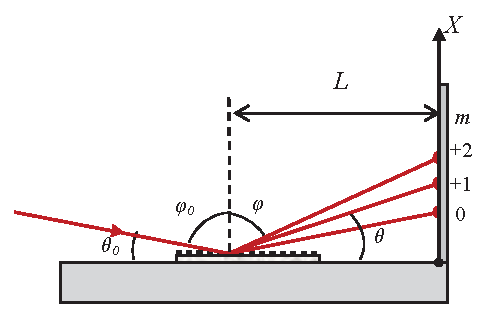
\includegraphics[width=0.45\textwidth]{pic1.png}}
		\caption[]{\label{fig:1} Схема установки для определения давления насыщенных паров.}
	\end{figure}

	Измерения проводятся на установке, изображенной на рис.1 . С помощью термостата A выставляется желаемая температура, и с помощью микроскопа C измеряется положение менисков ртути в U-образном манометре 15. Давление насыщенных паров считается как разность высот менисков ртути.
	\par
	Измерения проводятся в 2 этапа. В начале жидкость нагревается, а потом остужается. Это делается для того, чтобы посмотреть зависит ли давление насыщенных паров только от состояния жидкости или нет.
	
	\newpage
	
	\section{Выполнение}
	\begin{enumerate}
		\item Измерим разность уровней в ртутном U-образном манометре с помощью микроскопа и температуру по ртутному термометру. $\Delta H = H_{21} - H_{11} = 8.33\,см - 4.34\,см = 3.99\,см$. $T_0 = 19.1^\circ C$.
		
		\item Включим термостат. Начнём подогревать спирт ($\mu = 46\, ^{г}/_{моль}$) в калориметре, пропуская ток через нагреватель. Следим за тем, чтобы воздух все время перемешивал спирт. Измерим зависимость давления насыщенных паров от температуры.
		
		\begin{table}[h!] 
			\caption{Измерение при нагревании установки (красный цвет на графиках)}
			\begin{center}
				\begin{tabular}{|*{11}{l|}} \hline
					$T,\, ^\circ C$ & 19.1 & 21.1 & 23.1 & 25.1 & 27.1 & 29.1 & 31.1 & 33.1 & 35.1 & 37.1 \\ \hline
					$H,\, см$ & 3.99 & 4.33 & 4.83 & 5.47 & 6.15 & 6.87 & 7.75 & 8.55 & 9.29 & 10.69 \\ \hline
					$P,\, кПа$ & 5.33 & 5.78 & 6.45 & 7.30 & 8.21 & 9.17 & 10.35 & 11.41 & 12.40 & 14.27 \\ \hline
				\end{tabular}
			\end{center}
		\end{table}
	
		\begin{table}[h!] 
			\caption{Измерение при охлаждении установки (синий цвет на графиках)}
			\begin{center}
				\begin{tabular}{|*{11}{l|}} \hline
					$T,\, ^\circ C$ & 19.1 & 21.1 & 23.1 & 25.1 & 27.1 & 29.1 & 31.1 & 33.1 & 35.1 & 37.1 \\ \hline
					$H,\, см$ & 4.21 & 4.57 & 5.11 & 5.57 & 6.27 & 7.01 & 7.77 & 8.57 & 9.65 & 10.69 \\ \hline
					$P,\, кПа$ & 5.62 & 6.10 & 6.82 & 7.44 & 8.37 & 9.36 & 10.37 & 11.44 & 12.88 & 14.27 \\ \hline
				\end{tabular}
			\end{center}
		\end{table}
		
		\newpage 
		
		\item Построим график в координатах $P(T)$ (График №1).
		Заметим, что он вообще говоря не аппроксимируется прямой. Так что никаких прямых или кривых на графике проводить не будем.
		
		\begin{figure}[h!]
			\centering{\includegraphics[width=1\textwidth]{gr1.png}}
			\caption[]{\label{fig:2} График №1 $P(T)$ при нагреве и охлаждении}
		\end{figure}
	
		\newpage
		 
		\item Построим график в координатах $\ln P(T^{-1})$ (График №2):
		
		\begin{figure}[h!]
			\centering{\includegraphics[width=1\textwidth]{gr2.png}}
			\caption[]{\label{fig:3} График №2 $\ln P(T^{-1})$ при нагреве и охлаждении}
		\end{figure}
	
		$$\left(\dfrac{d(\ln P)}{d(1/T)}\right)_{нагр} = k_{нагр} = (-5007 \pm 6)\,К  \; \Rightarrow \; L_{нагр} = -\dfrac{R}{\mu} \dfrac{d(ln P)}{d(1/T)} = (903 \pm 1)\, ^{кДж}/_{кг}$$
		
		$$\left(\dfrac{d(\ln P)}{d(1/T)}\right)_{охл} = k_{охл} = (-4756 \pm  5)\, К \; \Rightarrow \; L_{охл} = -\dfrac{R}{\mu} \dfrac{d(ln P)}{d(1/T)} = (858 \pm 1)\, ^{кДж}/_{кг}$$
		
		$$\left(\dfrac{d(\ln P)}{d(1/T)}\right)_{ср} =<k>_{ср} = (-4882 \pm  125)\, К \; \Rightarrow \; L_{ср} = -\dfrac{R}{\mu} \dfrac{d(ln P)}{d(1/T)} = (881 \pm 26)\, ^{кДж}/_{кг}$$


\end{enumerate}

\section{Вывод}
	Полученное нами в результате эксперимента значения для удельной теплоты испарения спирта $L_{ср} = (881 \pm 26)\, ^{кДж}/_{кг}$, $\varepsilon_{L} \approx 3\%$. Само значение удельной теплоты испарения спирта получились, согласно справочным материалам, лежащим в пределах погрешности. $L^{*}_{20^\circ C} = 930^{кДж}/_{кг}$ $L^{*}_{78.5^\circ C} = 855^{кДж}/_{кг}$, наше значение, полученное при температурах $19--37^\circ C$ ложится в этот промежуток.
	При этом при нагреве $L_{нагр} = (903 \pm 1)\, ^{кДж}/_{кг}$, а при охлаждении $L_{охл} = (858 \pm 1)\, ^{кДж}/_{кг}$.

\end{document}